\documentclass{article}
\usepackage{amsmath}
\usepackage{amssymb}
\usepackage{graphicx}
\usepackage{float}
\usepackage{multirow}
\usepackage{verbatim}

\setlength{\parindent}{0em}
\setlength{\parskip}{1em}
\renewcommand{\arraystretch}{1.5}

\newcommand{\diff}{\mathop{}\!\mathrm{d}}
\newcommand{\prob}{\mathbb{P}}
\newcommand{\expect}{\mathbb{E}}

\title{Assignment 6}
\author{Joshua Hwang (44302650)}
\date{27 May}

\begin{document}
\maketitle

\section{One-step transition matrix}
Consider the one-step transition matrix,
\[
    P =
    \begin{bmatrix}
        0.1 & 0.1 & 0.8 \\
          0 & 0.6 & 0.4 \\
        0.3 & 0.7 &   0
    \end{bmatrix}
\]

\subsection{$\prob(X_1 = 3 | X_0 = 1)$}
We have the initial distribution as
\[
    \pi_0 =
    \begin{bmatrix}
        1 & 0 & 0
    \end{bmatrix}
\]

Thus we find the distribution at $X_1$,
\begin{align*}
    \pi_1
    &=
    \begin{bmatrix}
        1 & 0 & 0
    \end{bmatrix}
    \begin{bmatrix}
        0.1 & 0.1 & 0.8 \\
          0 & 0.6 & 0.4 \\
        0.3 & 0.7 &   0
    \end{bmatrix} \\
    &=
    \begin{bmatrix}
        0.1 & 0.1 & 0.8
    \end{bmatrix}
\end{align*}

Thus, $\prob(X_1 = 3 | X_0 = 1) = 0.8$ from the first column (which is $X_1$).

\subsection{$\expect[X_1 | X_0 = 1]$}
From the previous question we already have
\[
    \begin{bmatrix}
        0.1 & 0.1 & 0.8
    \end{bmatrix}
\]

Thus we compute, $0.1 \times 1 + 0.1 \times 2 + 0.8 \times 3 = 2.7$.

\subsection{$\prob(X_2 = 1 | X_0 = 2)$}
We apply the one-step transition matrix twice.
\begin{align*}
    \pi_2
    &=
    \begin{bmatrix}
        0 & 1 & 0
    \end{bmatrix}
    \begin{bmatrix}
        0.1 & 0.1 & 0.8 \\
          0 & 0.6 & 0.4 \\
        0.3 & 0.7 &   0
    \end{bmatrix}^2 \\
    &=
    \begin{bmatrix}
        0 & 1 & 0
    \end{bmatrix}
    \begin{bmatrix}
        0.25 & 0.63 & 0.12 \\
        0.12 & 0.64 & 0.24 \\
        0.03 & 0.45 & 0.52
    \end{bmatrix}^2 \\
    &=
    \begin{bmatrix}
        0.12 & 0.64 & 0.24
    \end{bmatrix}
\end{align*}

Thus, $\prob(X_2 = 1 | X_0 = 2) = 0.64$

\subsection{$\prob(X_1 = 1, X_2 = 2, X_3 = 3 | X_0 = 1)$}
Referring to the lecture notes we have the following formula derived from the
product rule and the Markov rule and expansion of conditional probablity.
\begin{align*}
    \prob(X_1 = 1, X_2 = 2, X_3 = 3 | X_0 = 1)
    &= \frac{\prob(X_0 = 1, X_1 = 1, X_2 = 2, X_3 = 3)}{\prob {X_0 = 1}} \\
    &= \frac{\prob(X_0 = 1) \prob(X_1 = 1 | X_0 = 1) \prob(X_2 = 2 | X_1 = 1) \prob(X_3 = 3 | X_2 = 2)}
        {\prob {X_0 = 1}} \\
    &= \prob(X_1 = 1 | X_0 = 1) \prob(X_2 = 2 | X_1 = 1) \prob(X_3 = 3 | X_2 = 2)
\end{align*}

Performing a single multiplication of our one-step transition matrix will move
us from time $i$ to time $i+1$. Thus, e now calculate each probability
in the same way as the first question.
\begin{align*}
    \pi_1
    &=
    \begin{bmatrix}
        1 & 0 & 0
    \end{bmatrix}
    \begin{bmatrix}
        0.1 & 0.1 & 0.8 \\
          0 & 0.6 & 0.4 \\
        0.3 & 0.7 &   0
    \end{bmatrix} \\
    &=
    \begin{bmatrix}
        0.1 & 0.1 & 0.8
    \end{bmatrix}
\end{align*}
Thus, $\prob(X_1 = 1 | X_0 = 1) = 0.1$

\begin{align*}
    \pi_2
    &=
    \begin{bmatrix}
        1 & 0 & 0
    \end{bmatrix}
    \begin{bmatrix}
        0.1 & 0.1 & 0.8 \\
          0 & 0.6 & 0.4 \\
        0.3 & 0.7 &   0
    \end{bmatrix} \\
    &=
    \begin{bmatrix}
        0.1 & 0.1 & 0.8
    \end{bmatrix}
\end{align*}
Thus, $\prob(X_2 = 2 | X_1 = 1) = 0.1$

\begin{align*}
    \pi_3
    &=
    \begin{bmatrix}
        0 & 1 & 0
    \end{bmatrix}
    \begin{bmatrix}
        0.1 & 0.1 & 0.8 \\
          0 & 0.6 & 0.4 \\
        0.3 & 0.7 &   0
    \end{bmatrix} \\
    &=
    \begin{bmatrix}
        0 & 0.6 & 0.4
    \end{bmatrix}
\end{align*}
Thus, $\prob(X_3 = 3 | X_2 = 2) = 0.4$

Note we did not have to perform these calculations since each row vector
was extracting its respective row from the matrix from which we could have
further extracted the relevant cell.

Now we may calculate our final result,
\begin{align*}
    \prob(X_1 = 1 | X_0 = 1) \prob(X_2 = 2 | X_1 = 1) \prob(X_3 = 3 | X_2 = 2)
    &= 0.1 \times 0.1 \times 0.4 \\
    &= 0.004
\end{align*}

Thus, $\prob(X_1 = 1, X_2 = 2, X_3 = 3 | X_0 = 1) = 0.004$

\subsection{The stationary distribution}
The stationary distribution satisfies the following $\pi = \pi P$.
We solve via,
\begin{align*}
    \pi &= \pi P \\
    \pi I &= \pi P \\
    \pi (P - I) &= 0 \\
    (P - I)^T \pi^T &= 0^T \\
\end{align*}

We could either calculate the appropriate vector through Gaussian elimination
or, in this case, use a program to calculate the nullspace (kernel) of our
matrix.
\begin{verbatim}
import numpy as np
from numpy.linalg import svd

def nullspace(A, atol=1e-13, rtol=0):
    A = np.atleast_2d(A)
    u, s, vh = svd(A)
    tol = max(atol, rtol * s[0])
    nnz = (s >= tol).sum()
    ns = vh[nns:].conj().T
    return ns

A = np.matrix('0.1 0.1 0.8; 0 0.6 0.4; 0.3 0.7 0')
p = nullspace(np.transpose(A - np.identity(3)))
p = p/sum(p)
print(p.T)
\end{verbatim}

From this we find the vector (to 4 decimal places)
\[
    \begin{bmatrix}
        0.1053 & 0.5789 & 0.3158
    \end{bmatrix}
\]

\subsection{$\expect[X_2 | X_0 = 2]$}
Recall the section where we calculated $\prob(X_2 = 1 | X_0 = 2)$.
We got the following final vector
\[
    \begin{bmatrix}
        0.12 & 0.64 & 0.24
    \end{bmatrix}
\]

Thus the expectation from this vector is,
$0.12 \times 1 + 0.64 \times 2 + 0.24 \times 3 = 2.12$.

\subsection{$\lim_{n \to \infty} P^n$}
All rows of $P^\infty$ are equal to the limiting distribution $\pi$.
Since we've calculated the limiting distribution already
\[
    \begin{bmatrix}
        0.1053 & 0.5789 & 0.3158 \\
        0.1053 & 0.5789 & 0.3158 \\
        0.1053 & 0.5789 & 0.3158
    \end{bmatrix}
\]

\section{Mouse maze}
\subsection{Determine the one-step transition matrix}
From the assumptions stated we may create a transition matrix.
A one-step transition matrix is constructed from transitions
from a state (columns) to a state (rows). From these we get the following,
\[
    \begin{bmatrix}
        0 & 0.5 & 0.5 & 0 & 0 & 0 \\
        1 & 0 & 0 & 0 & 0 & 0 \\
        0.5 & 0 & 0 & 0.5 & 0 & 0 \\
        0 & 0 & 0.33 & 0 & 0.33 & 0.33 \\
        0 & 0 & 0 & 0.5 & 0 & 0.5 \\
        0 & 0 & 0 & 0.5 & 0.5 & 0 \\
    \end{bmatrix}
\]

Note the $0.33$ is actually $\frac{1}{3}$ I'm just lazy.

\subsection{Calculate a probability}
\begin{verbatim}
A = np.matrix('0 0.5 0.5 0 0 0; 1 0 0 0 0 0; 0.5 0 0 0.5 0 0; \
    0 0 0.333333333333 0 0.3333333333333333333 0.333333333333333333; \
    0 0 0 0.5 0 0.5; 0 0 0 0.5 0.5 0')

print(np.matrix('0 0 0 1 0 0')*A**7)

------------------------------- Output ---------------------------------------
matrix([[0.05555556, 0.109375  , 0.2193287 , 0.21875   , 0.19849537,
         0.19849537]])
\end{verbatim}

The answer is 0.19849537

The second answer is 0.1666666666666 which is 1/6

\section{Monte Carlo}
\subsection{Find pdf of $X$}
This random variable is equivalent to a binomial distribution with a
probability $p$ of landing inside the circle. The probability that a single
point lands in the circle, given any random point in the unit square is
determined by the proportion of area taken up by a circle (diameter 1)
in regards to the unit square
(which is luckily ${}^\pi/_4$ and 1 respectively).
\[
    p = \frac{\pi}{4}
\]

Thus our probability is
\begin{align*}
    f(x) = \prob(X=x) &= {}^nC_x p^x (1-p)^{n-x} \\
    &= {}^nC_x \frac{\pi}{4}^x (1-\frac{\pi}{4})^{n-x}
\end{align*}

\subsection{Find $4X/n$ for large $n$}
For large $n$ a binomial distribution approximates a normal distribution
of the form,
\[
    N(np, np(1-p))
\]

Since we're multiplying our original $X$ by $\frac{4}{n}$ our
normal distribution approximation will become
\begin{align*}
    \frac{4}{n} \times N\left(n\frac{\pi}{4}, n\frac{\pi}{4}
        \left(1-\frac{\pi}{4}\right)\right)
    &= \frac{4}{n} \times \left(n\frac{\pi}{4}
        + \sqrt{n\frac{\pi}{4}\left(1-\frac{\pi}{4}\right)} N(0, 1))\right) \\
    &= \pi + \sqrt{\frac{4\pi}{n}\left(1-\frac{\pi}{4}\right)} N(0, 1) \\
    &= N(\pi, \frac{4\pi}{n}\left(1-\frac{\pi}{4}\right))
\end{align*}

Thus our approximate distribution is a normal distribution with
a mean $\pi$ and variance $\frac{4\pi}{n}\left(1-\frac{\pi}{4}\right)$.

\subsection{95\% confidence interval}
We first create our estimated mean for $\pi$.
\[
    4 \times \frac{756}{1000} = 3.024
\]

It follows that our estimated variance is,
\begin{align*}
    \frac{4\pi}{n}\left(1-\frac{\pi}{4}\right)
    &= \frac{4\times3.024}{n}\left(1-\frac{3.024}{4}\right) \\
    &= 0.002951 && \text{Four significant figures} \\
    \sqrt{0.002951} &= 0.05433 && \text{Standard deviation} \\
\end{align*}

From here we generate our confidence interval,
(Note: we use $n=1$ here since this is the number of trials, different to the
$n$ in our equations for $X$)
\begin{align*}
    \bar{X} \pm z \frac{S}{\sqrt{n}} &= \bar{\pi} \pm z \frac{0.05433}{\sqrt{1}} \\
    &= 3.024 \pm z 0.05433 \\
    &= 3.024 \pm 1.96 \times 0.05433 \\
    &= 3.024 \pm 0.1065 \\
\end{align*}

Note, our confidence interval of 95\% does not contain the actual value
of $\pi$. This could just be an unlucky trial, given a more generous
confidence interval we would contain the actual value of $\pi$.

\section{Markov chain}
We first simplify our recursive relationship,
\begin{align*}
    X_{n+1} &= \frac{nX_n + Z_{n+1}}{n+1} \\
    &= \frac{n\frac{(n-1)X_{n-1} + Z_{n}}{n} + Z_{n+1}}{n+1} \\
    &= \frac{(n-1)X_{n-1} + Z_{n} + Z_{n+1}}{n+1} \\
    \vdots \\
    &= \frac{\text{Stuff}X_{0} + Z_1 + \dots + Z_{n} + Z_{n+1}}{n+1} \\
    &= \frac{Z_1 + \dots + Z_{n} + Z_{n+1}}{n+1} \\
\end{align*}

Since we know our initial condition is $X_0 = 0$ we obtain the previously
stated relationship for each $X$.

\subsection{Find expectation and variance}
Since
\[
    \expect(X + Y) = \expect X + \expect Y
\]
from the proofs in the lecture notes,
we can employ this to find our expectations.
\begin{align*}
    \expect X_n &= \expect \frac{Z_1 + \dots + Z_{n}}{n} \\
    &= \frac{\expect Z_1 + \dots + \expect Z_{n}}{n} \\
    &= \frac{0}{n} \\
    &= 0 \\
\end{align*}

Since
\[
    Var(X + Y) = Var(X) + Var(Y) + 2Cov(X,Y)
\]
but since $X$ and $Y$ will be independent we will have $Cov(X,Y) = 0$.

\begin{align*}
    Var(X_n) &= Var\left(\frac{Z_1 + \dots + Z_{n}}{n}\right) \\
    &= \frac{Var(Z_1) + \dots + Var(Z_{n})}{n^2} \\
    &= \frac{1 + \dots + 1}{n^2} \\
    &= \frac{n}{n^2} \\
    &= \frac{1}{n} \\
\end{align*}

\subsection{The probability distribution of $X_n$}
Since each $X_n$ is just a sum of normal random variables (and division by a
constant) the probability will be a normal distribution with mean of 0 and
variance $\frac{1}{n}$.
\[
    X_n \sim N\left(0, \frac{1}{n}\right)
\]

\subsection{Find probability}
As $n \to \infty$ the variance of $X_n$ reduces, $\frac{1}{n}$. When
variance $\to 0$ the only possible value is the mean which is $0$.
Thus no other value $X_n > 0$ is possible,
$\prob (X_n > \epsilon) = 0$.

\subsection{Simulation}
The code below was run,
\verbatiminput{q4.py}

and the following outputs were taken,
\begin{figure}[H]
    \centering
    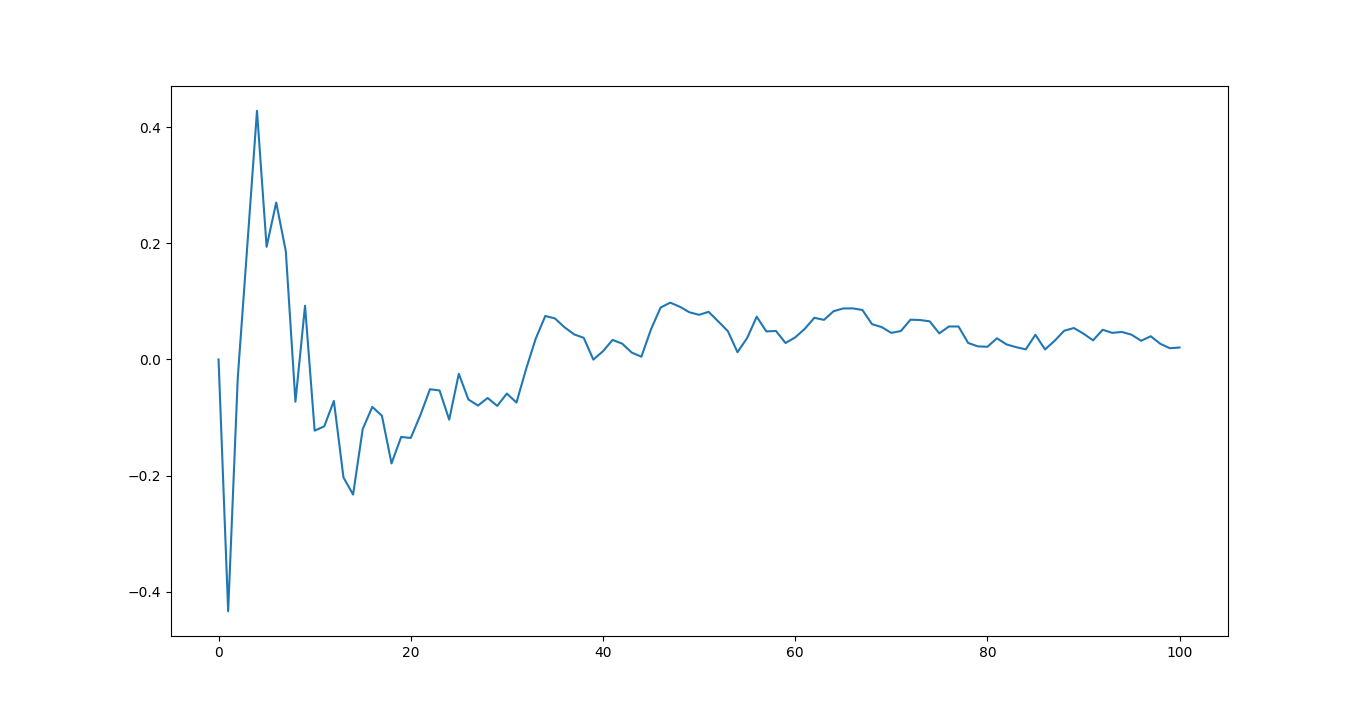
\includegraphics[width=5in]{figure1.png}
\end{figure}
\begin{figure}[H]
    \centering
    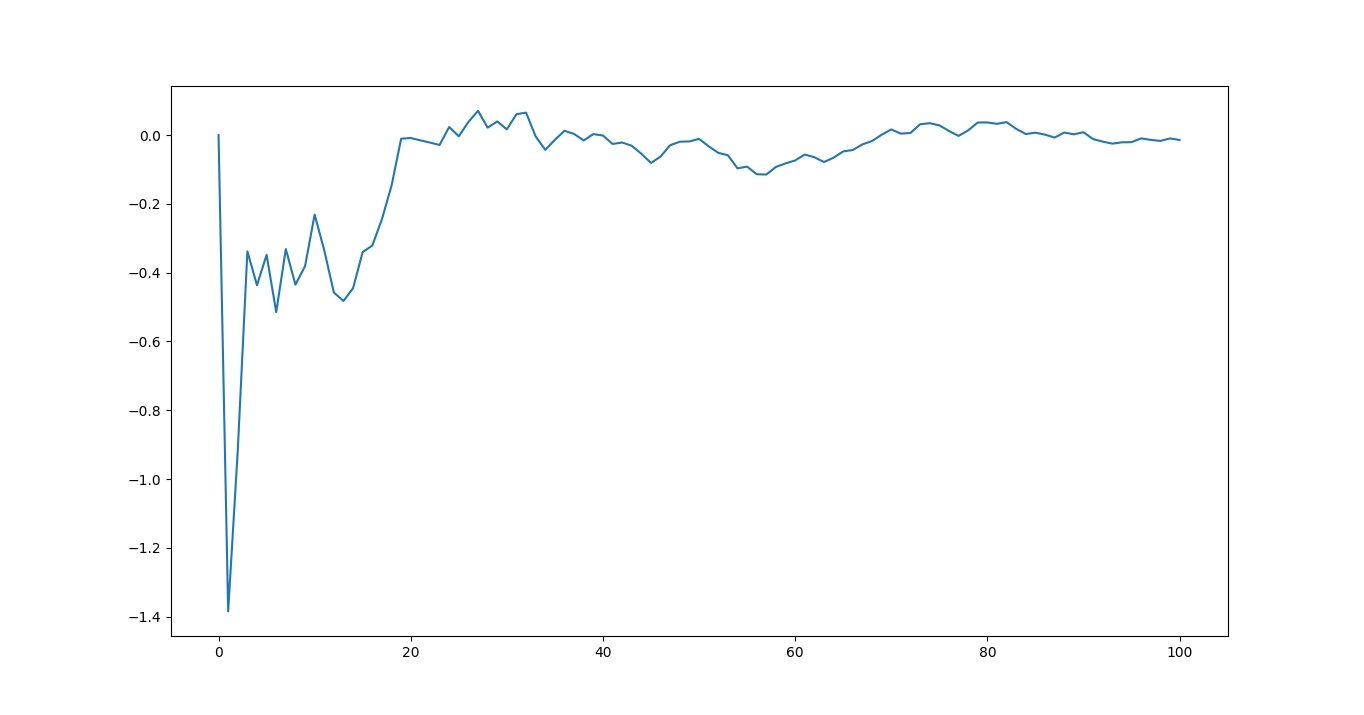
\includegraphics[width=5in]{figure2.png}
\end{figure}

\end{document}
